%!TEX root = main.tex
\chapter{Results}
\label{chap:results}
In this chapter we will show and discuss the results of the work we have reached in this thesis.

We will start by looking at the train and test sets of the four dataset (see \autoref{tab:model_delimitation} and below) and describe what we did about class imbalance. Then we describe and interpret our results and we end the chapter with a brief summary of our findings. 

From \autoref{chap:methods} we have found the following datasets and model pairs based on the available data (see also \autoref{tab:model_overview} and \autoref{tab:model_delimitation}):
\begin{enumerate}
\item Test data
\begin{enumerate}
\item without user-filtering \\\textbf{Model pair: TP-1}
\item with user-filtering using cross-occupancy of 40\% \\\textbf{Model pair: TP-2}
\end{enumerate}
\item Production data
\begin{enumerate}
\item without user-filtering \\\textbf{Model pair: PP-1}
\item with user-filtering using cross-occupancy of 10\% \\\textbf{Model pair: PP-1}
\end{enumerate}
\end{enumerate}


For our test data without user-filtering we found a training set with 1798 negative samples (did not meet) and 9203 positive samples (did meet). In our test set we found a more moderate 5513 negative samples (did not meet) and 1674 positive samples (did meet).

Using test data with user-filtering in just September we found a training set with 118 that did not meet and 95 that did meet. The test set consisted of 151 that did not meet and 98 that did meet. 

Using production data without user-filtering we found 5585 that did not meet and 10907 that did meet for our training set, for our test set we found 9148 that did not meet and 10028 that did meet.

Using production data with user-filtering we found 403 that did not meet and 4533 that did meet for our train set and 402 that did not meet and 4630 that did meet for our test set.

The datasets composed from the test data have more negative samples than positive samples. In TP-1 the difference is more pronounced than in TP-2, except for the training set. In the production data, we have the opposite. Here we have more positive samples than negative. \\
This shows that for some of the datasets we have a class imbalance problem. Due to this, the Logistic Regression classifier we trained initially predicted the largest prevalent class, in our training dataset. The next section explains this problem and how we dealt with it. 


\section{Class Imbalance Problem}
\label{sec:class_imbalance_problem}
The Class Imbalance Problem is when the total number of samples for one class greatly exceeds the number of samples for a different class. A number of techniques can be used to handle the class imbalance problem, two of the most common techniques are called \textit{oversampling} and \textit{undersampling}\cite{tan2006introduction}. In oversampling you sample the minor sample with replacement until there is an equal number of positive and negative samples. In undersampling you randomly sample from the major class $N$ times where $N$ is the number of minor classes. The drawbacks of undersampling is the loss of information in the dataset, as samples from the major class is removed. The advantage is, that all of the minority class is maintained, where in oversampling we create duplicate copies of the minority class, which can cause overfitting.
We will train our models with and without undersampling our datasets to see how it affects our performance metrics.

\section{Performance metrics}
\label{sec:performance_metrics}
We utilize the precision and recall metrics for evaluating the performance of our models as well as AUC of the ROC Curve.

\subsection{Receiver Operating Characteristic (ROC)}
The Receiver Operating Characteristic or ROC in short, illustrates the performance of a binary classifier in terms of the true positive rate (TPR, also called recall) plotted against the false positive rate (FPR) at different discrimination thresholds. As points on the ROC-curve represents different thresholds with an associated (TPR,FPR) pair, it allows us to see different trade-offs between TPR and FPR. The ROC curve is useful for comparing the relative performance of different classifiers\cite{tan2006introduction} The area under the curve (AUC) represents the probability that a classifier will rank a random positive sample higher than a negative sample, assuming positive ranks higher. An AUC of 0.5 would mean the model would just randomly guess the class of each sample. We will use the ROC AUC as a metric for comparing our different models.

In Figure \ref{fig:rocs} we have plotted the ROC curve and ROC AUC for the different model pairs, we have also plotted the curve of a randomly guessing classifier for comparison. Figure \ref{fig:rocs_undersampling} shows the same models performance, where the datasets most prevalent class have been undersampled. We used randomized search to find the optimal hyper-parameters in the Random Forest models, choosing from \textit{gini} or \textit{entropy} as split criterion and $1-9$ max features for each split. The randomized search runs for 20 iterations where each iteration performs a 3-fold cross-validation to validate the parameters of the model, we used ROC AUC as the scoring function. When the best parameters for the model are found, 2-fold cross-validation is performed to validate the model.

Looking at Figure \ref{fig:rocs} we see the Random Forest model is higher than baseline for every case. Looking at the case of using all users, the difference is miniscule, but using the users with a cross-occupancy threshold makes it more pronounced. Comparing test with production the outputs look similar.

\begin{figure}[H]
    \hspace*{-1.0cm}
    \centering
    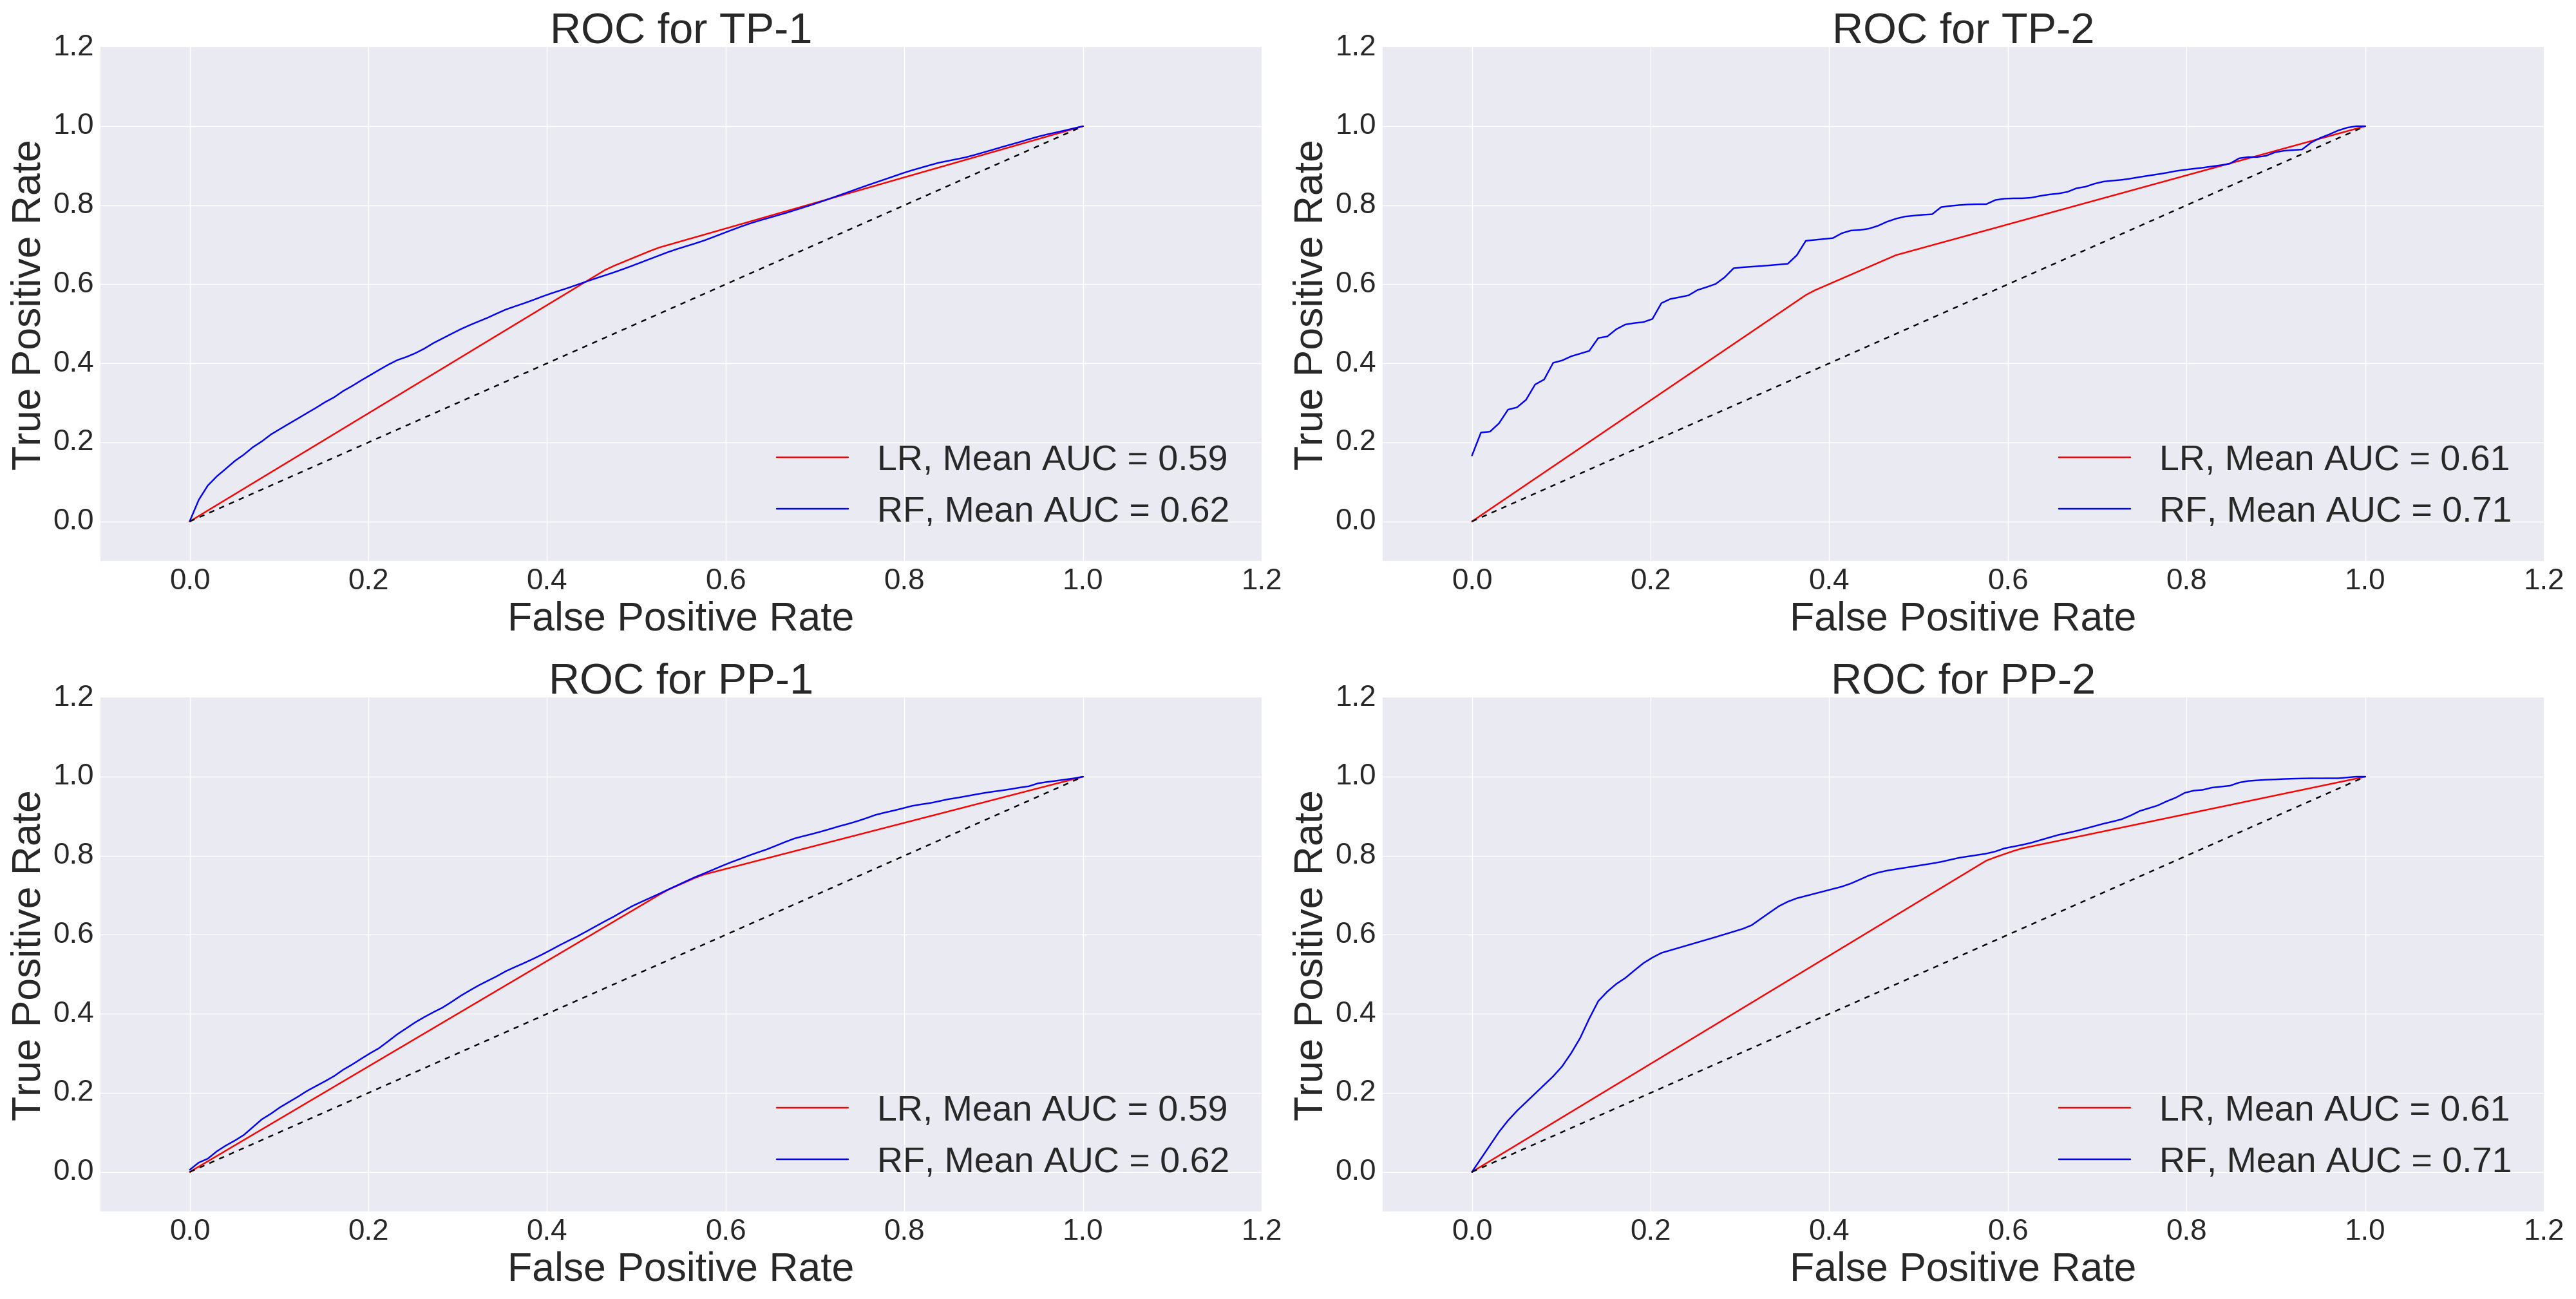
\includegraphics[scale=0.15]{ROCS}
    \caption{Mean ROC AUC of Logistic Regression (LR) and Random Forest (RF) in the four model-pairs (TP-1, TP-2, PP-1, PP-2) using randomized search for hyper-parameter optimization (internal loop with 3-fold cross-validation) and 2-fold cross-validation. }
    \label{fig:rocs}
\end{figure}

Looking at Figure \ref{fig:rocs_undersampling} we see similar results as without undersampling.

\begin{figure}[H]
    \hspace*{-1.0cm}
    \centering
    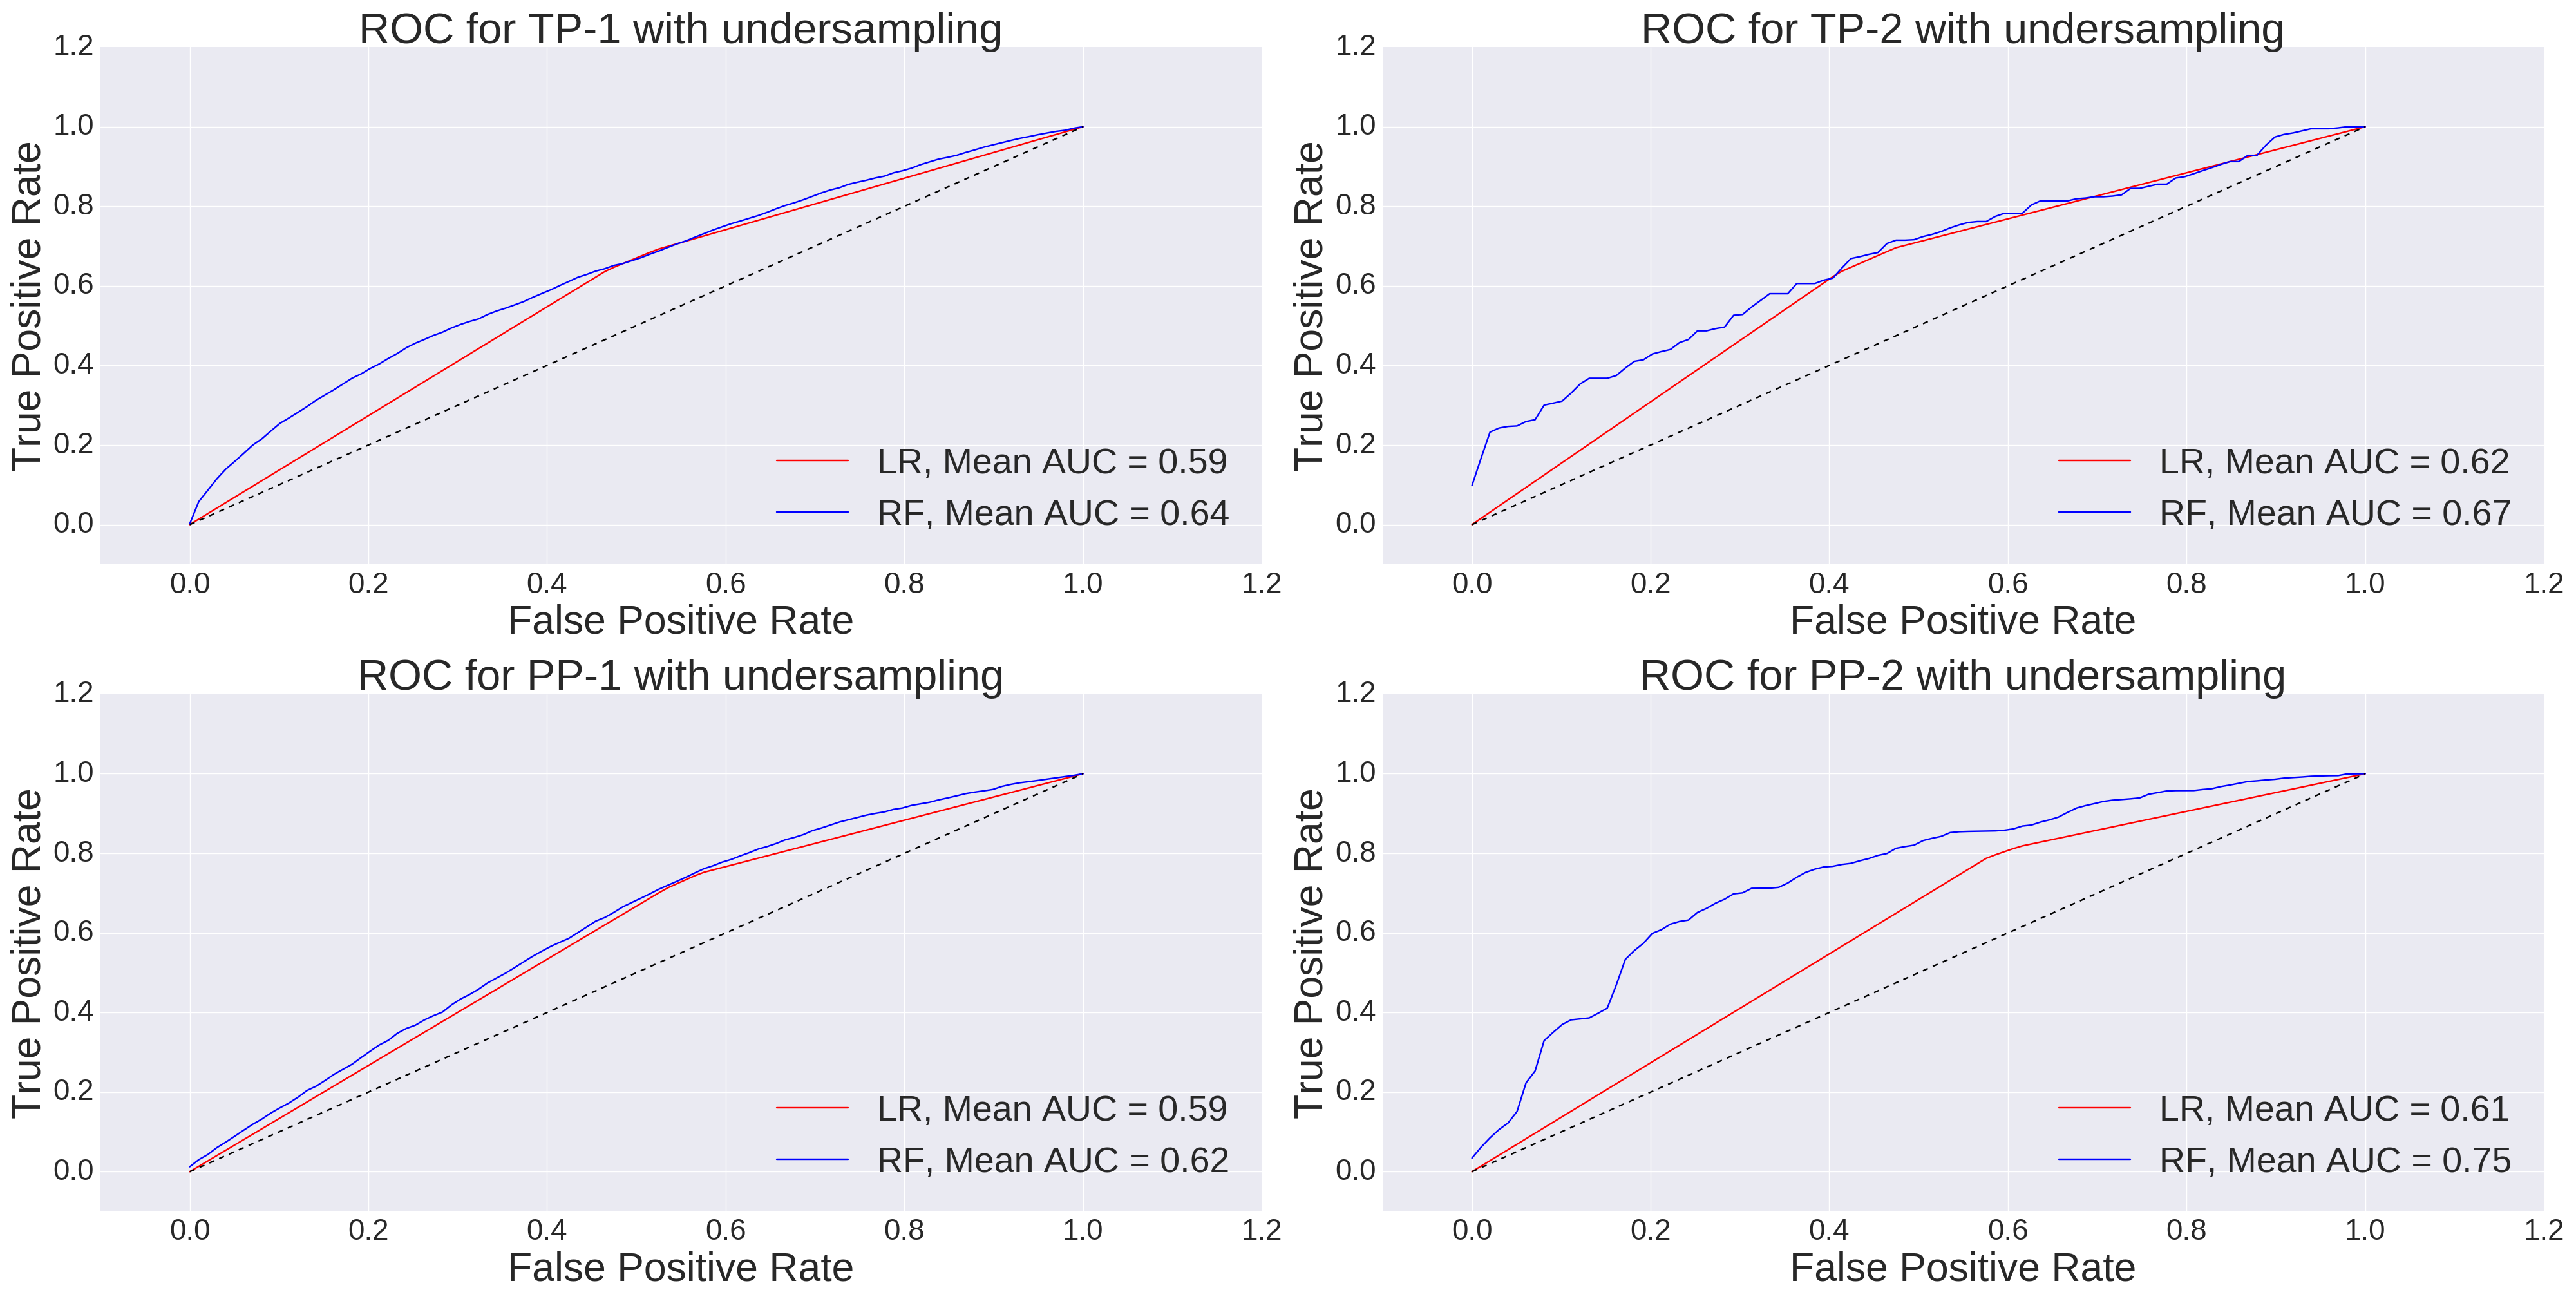
\includegraphics[scale=0.15]{ROCS_undersampling}
    \caption{Mean ROC AUC of Logistic Regression (LR) and Random Forest (RF) in the four model-pairs (TP-1, TP-2, PP-1, PP-2) using randomized search for hyper-parameter optimization (internal loop with 3-fold cross-validation) and 2-fold cross-validation, and with undersampling of the most prevalent class}
    \label{fig:rocs_undersampling}
\end{figure}

Comparing Figure \ref{fig:rocs} and \ref{fig:rocs_undersampling} it seems undersampling does not make a significant difference for performance between the models.

Overall we find the Random forest provides a higher ROC AUC score than the baseline model and thus that it does a better job of predicting classes, albeit not by much.

In the next section we will look at the performance of the models in terms of the precision and recall scores of the positive class.  

\subsection{Precision and Recall}
We will use the metrics Precision and Recall to further evaluate the performance of our models.

Precision and Recall are defined using the following measures: True positive ($TP$), the number of records predicted to be positive which really are positive. False positive ($FP$), the number of records predicted to be positive but are negative. Lastly, $FN$ which is false negative, the number of records predicted to be negative which actually are positive.

Precision or the positive predictive value (PPV) is a metric that measures the number of a given class that are correctly identified in proportion to the number of classes that are predicted to be that class.

Recall, or the true positive rate (TPR), is a metric that measures the number of a given class that are correctly identified as that class. PPV and TPR is defined in \autoref{eq:precision} and \autoref{eq:recall} respectively.

\begin{equation}
\label{eq:precision}
PPV=\frac{TP}{TP+FP}
\end{equation}

\begin{equation}
\label{eq:recall}
TPR=\frac{TP}{TP+FN}
\end{equation}

As a summary we have the $F_1$ score which is the harmonic mean of the precision and recall. Since the score tend to be closer to the lowest value (of precision and recall), a high $F_1$ score ensures precision and recall to be reasonably high\cite{tan2006introduction}. 
The $F_1$ score is defined in Equation \ref{eq:f1_score}

\begin{equation}
\label{eq:f1_score}
F_1=\frac{2 \cdot TP}{2 \cdot TP+FP+FN}
\end{equation}

In Table \ref{table:models_performance_report} and \ref{table:models_performance_report_undersampling} we can see the performance metrics of the different classifiers for the positive class (did meet), in the dataset without and with undersampling respectively.

\begin{table}[H]
\centering
\begin{tabular}{|c|c|c|c|c|c|c|c|}
\hline
\textbf{Model} & \textbf{PPV} & \textbf{TPR} & \textbf{$F_1$-score}   \\
\specialrule{.20em}{.0em}{.0em}
LR in TP-1    & 0.25 & 0.67 & 0.37 \\
\hline
RF in TP-1    & 0.47 & 0.15 & 0.23 \\
\specialrule{.15em}{.0em}{.0em} 
LR in TP-2    & 0.53 & 0.68 & 0.59 \\
\hline
RF in TP-2    & 0.54 & 0.52 & 0.53 \\
\specialrule{.15em}{.0em}{.0em}
LR in PP-1    & 0.66 & 0.74 & 0.70 \\
\hline
RF in PP-1    & 0.65 & 0.61 & 0.63 \\
\specialrule{.15em}{.0em}{.0em}
LR in PP-2    & 0.94 & 0.81 & 0.87 \\
\hline
RF in PP-2    & 0.93 & 0.99 & 0.96 \\
\hline
\end{tabular}
\caption{Models performance metrics for the positive class (did meet) without undersampling}
\label{table:models_performance_report}
\end{table}

Looking at Table \ref{table:models_performance_report} we find the recall is higher for the baseline for all of the datasets except for PP-2.
The precision values for the different models have similar values for each dataset.

Looking at the $F_1$ score which considers both precision and recall we see that each model pair performs better than the last when considering the datasets in sequence. This might be because the users of the production data are less homogeneous than the users in the test data and biases or noise which might be inherent in the test data might not be present in the production data. Furthermore filtering users on cross-occupancy, ensured the users had data in all periods and thus reduce the number of cases where they might have a co-occurrence, but fails to show it due to lack of location updates.

The $F_1$ score also shows that the baseline is better in all the pairs except for PP-2. This is surprising but might be because some of our features are not important to the classification task and presents themselves as noise.

\begin{table}[H]
\centering
\begin{tabular}{|c|c|c|c|c|c|c|c|}
\hline
\textbf{Model} & \textbf{PPV +} & \textbf{TPR +} & \textbf{f-score}    \\
\specialrule{.20em}{.0em}{.0em}
LR in TP-1    & 0.25 & 0.67 & 0.37 \\
\hline
RF in TP-1    & 0.28 & 0.53 & 0.37 \\
\specialrule{.15em}{.0em}{.0em} 
LR in TP-2    & 0.53 & 0.68 & 0.59 \\
\hline
RF in TP-2    & 0.53 & 0.62 & 0.57 \\
\specialrule{.15em}{.0em}{.0em}
LR in PP-1    & 0.66 & 0.74 & 0.70 \\
\hline
RF in PP-1    & 0.66 & 0.56 & 0.61 \\
\specialrule{.15em}{.0em}{.0em}
LR in PP-2    & 0.94 & 0.81 & 0.87 \\
\hline
RF in PP-2    & 0.95 & 0.89 & 0.92 \\
\hline
\end{tabular}
\caption{Models performance metrics for the positive class (did meet) with undersampling}
\label{table:models_performance_report_undersampling}
\end{table}

In Table \ref{table:models_performance_report_undersampling} with undersampling we see similar values for precision and recall as found without undersampling.
Looking at the $F_1$ score we see the highest score coming from the RF model in PP-2, but values are higher from the baseline models for the other datasets.

It seems undersampling does not affect the scores notably with respect to the positive class, perhaps except for the RF model in TP-1.

\subsection{Feature importance}
The Random Forest model allows for finding the relative importance of the different features. The depth of a feature in the trees can be used to determine importance, as features at the top of the tree contributes to the prediction decision over a larger fraction of samples. The average is then computed from each tree in the forest to obtain the final feature importances.\\
Figure \ref{fig:feature_importances_pp2} shows the mean of the feature importances of the random forest of PP2 and \autoref{fig:feature_importances_tp2} shows it for TP-2. \\

\begin{figure}[H]
    \hspace*{-1.0cm}
    \centering
    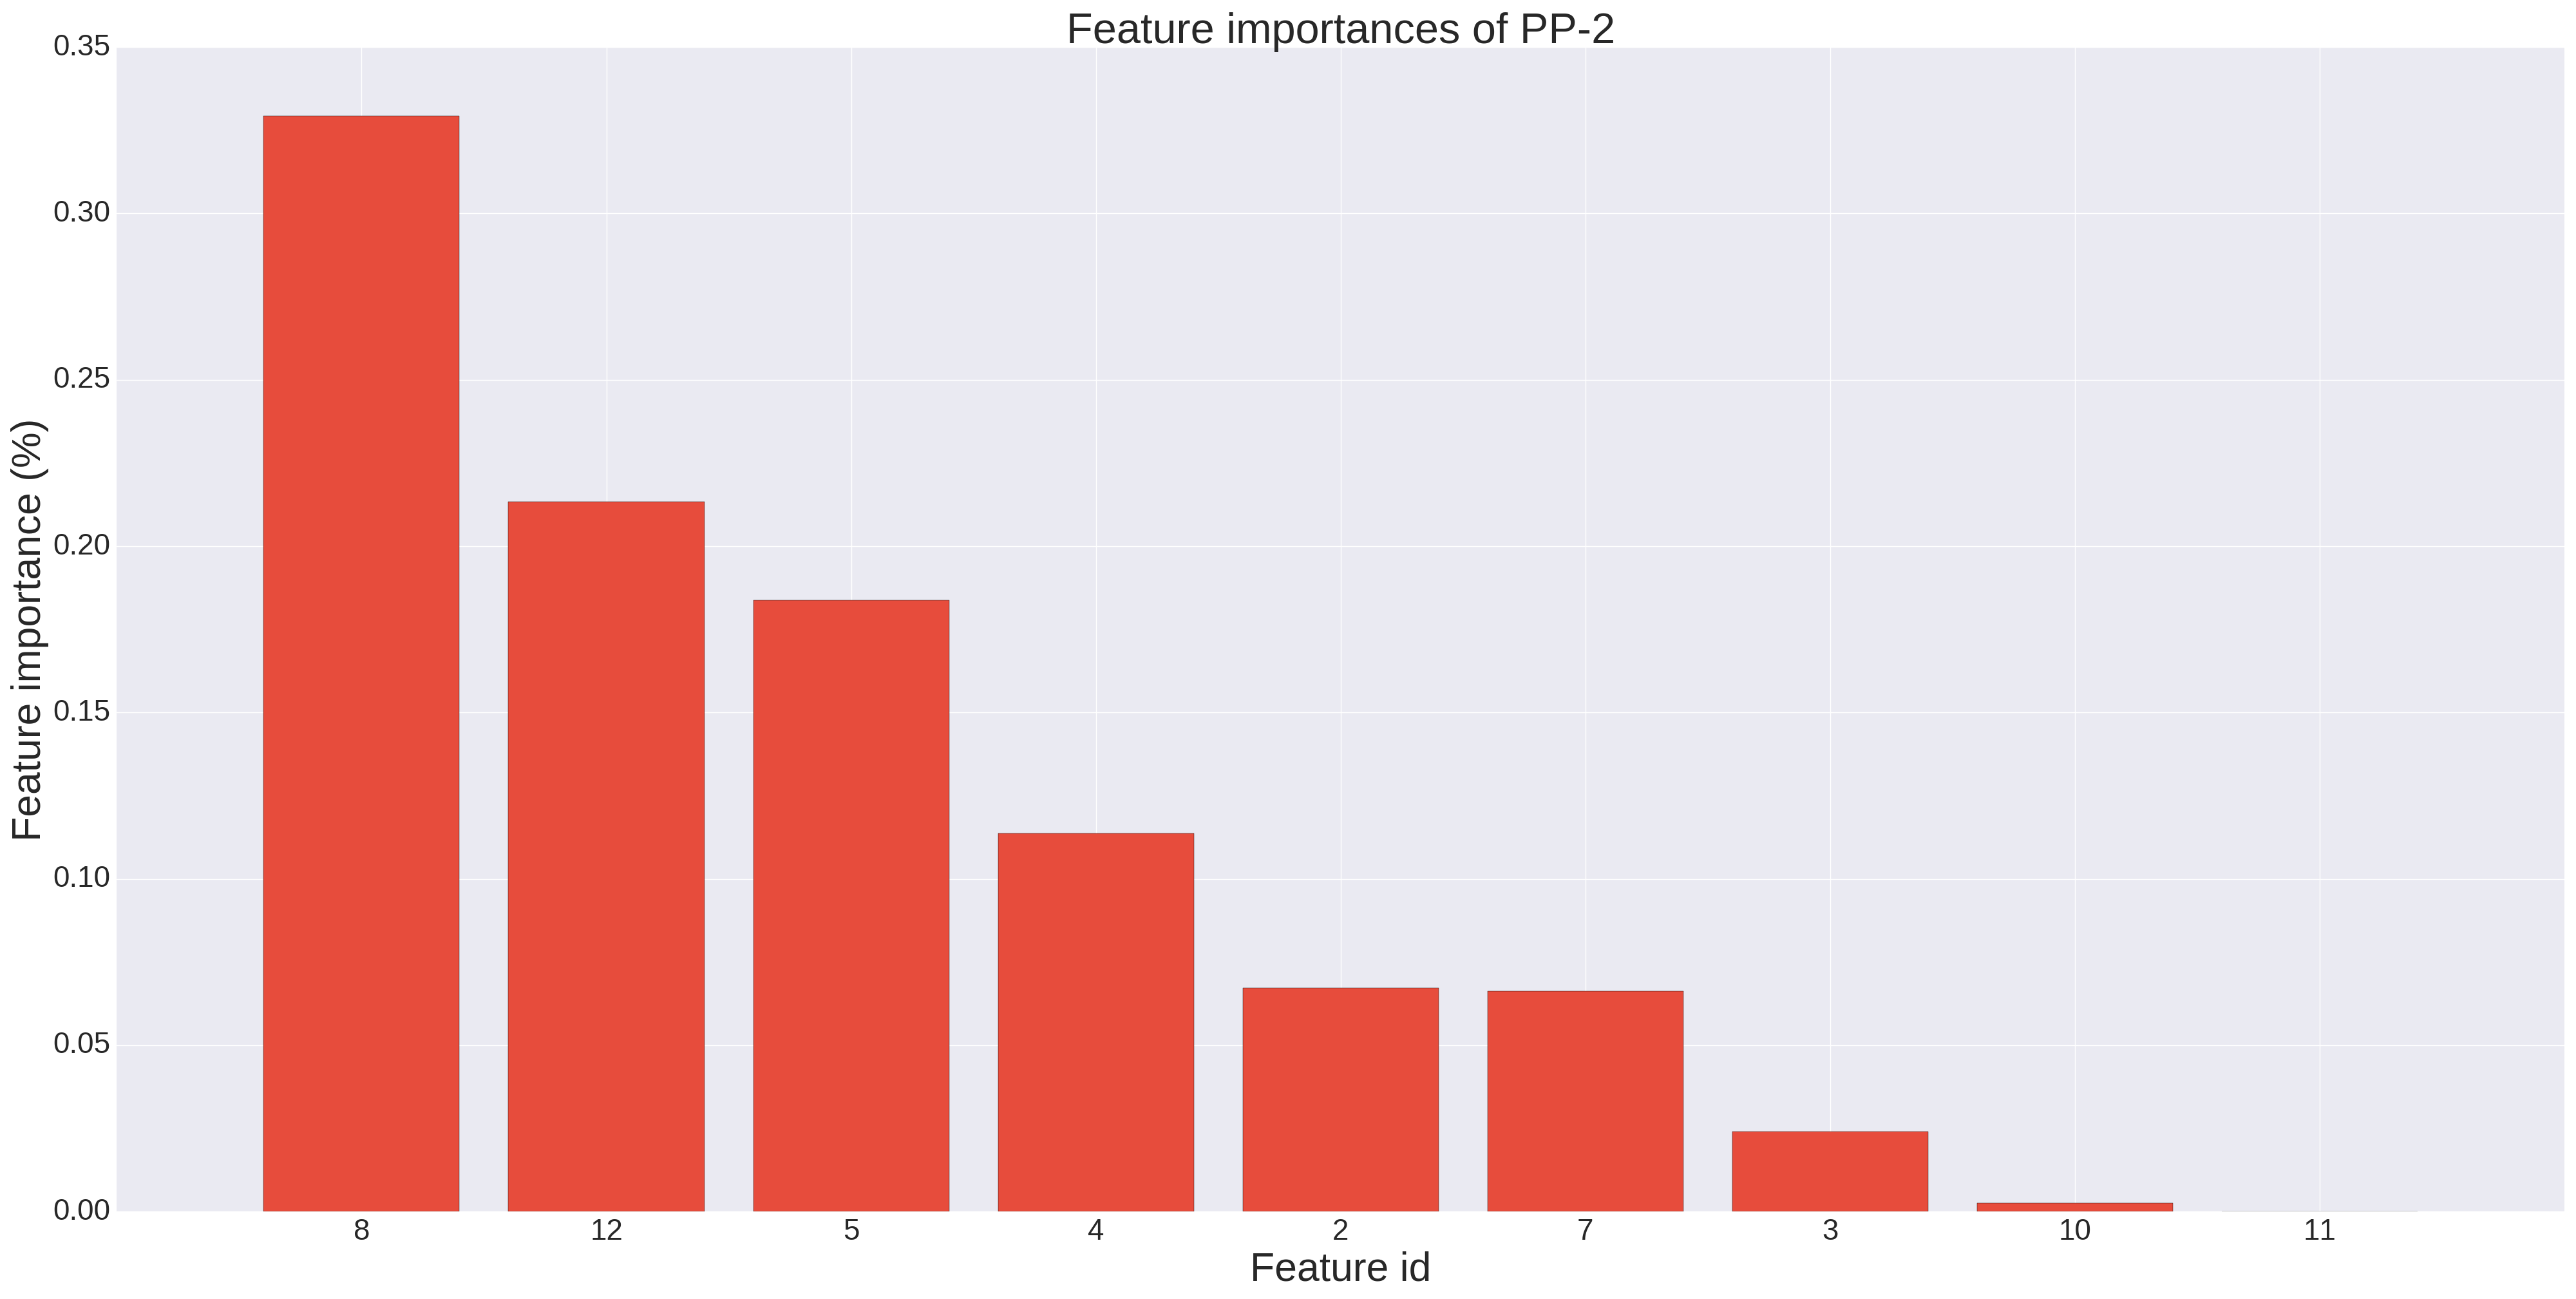
\includegraphics[scale=0.10]{feature_importance_PP2}
    \caption{Feature importances of random forest for PP2}
    \label{fig:feature_importances_pp2}
\end{figure}
We can see for PP-2, the features which contribute most are features 8 (mutual co-occurrences), 12 (specificity), 5 (co-occurrences weighted), 4 (weighted frequency), 2 (diversity), 7 (number of co-occurrences), 3 (unique co-occurrences). Feature 10 (number of evenings) contributes very little and 11 (number of weekends) seems to have no variance.

\begin{figure}[H]
    \hspace*{-1.0cm}
    \centering
    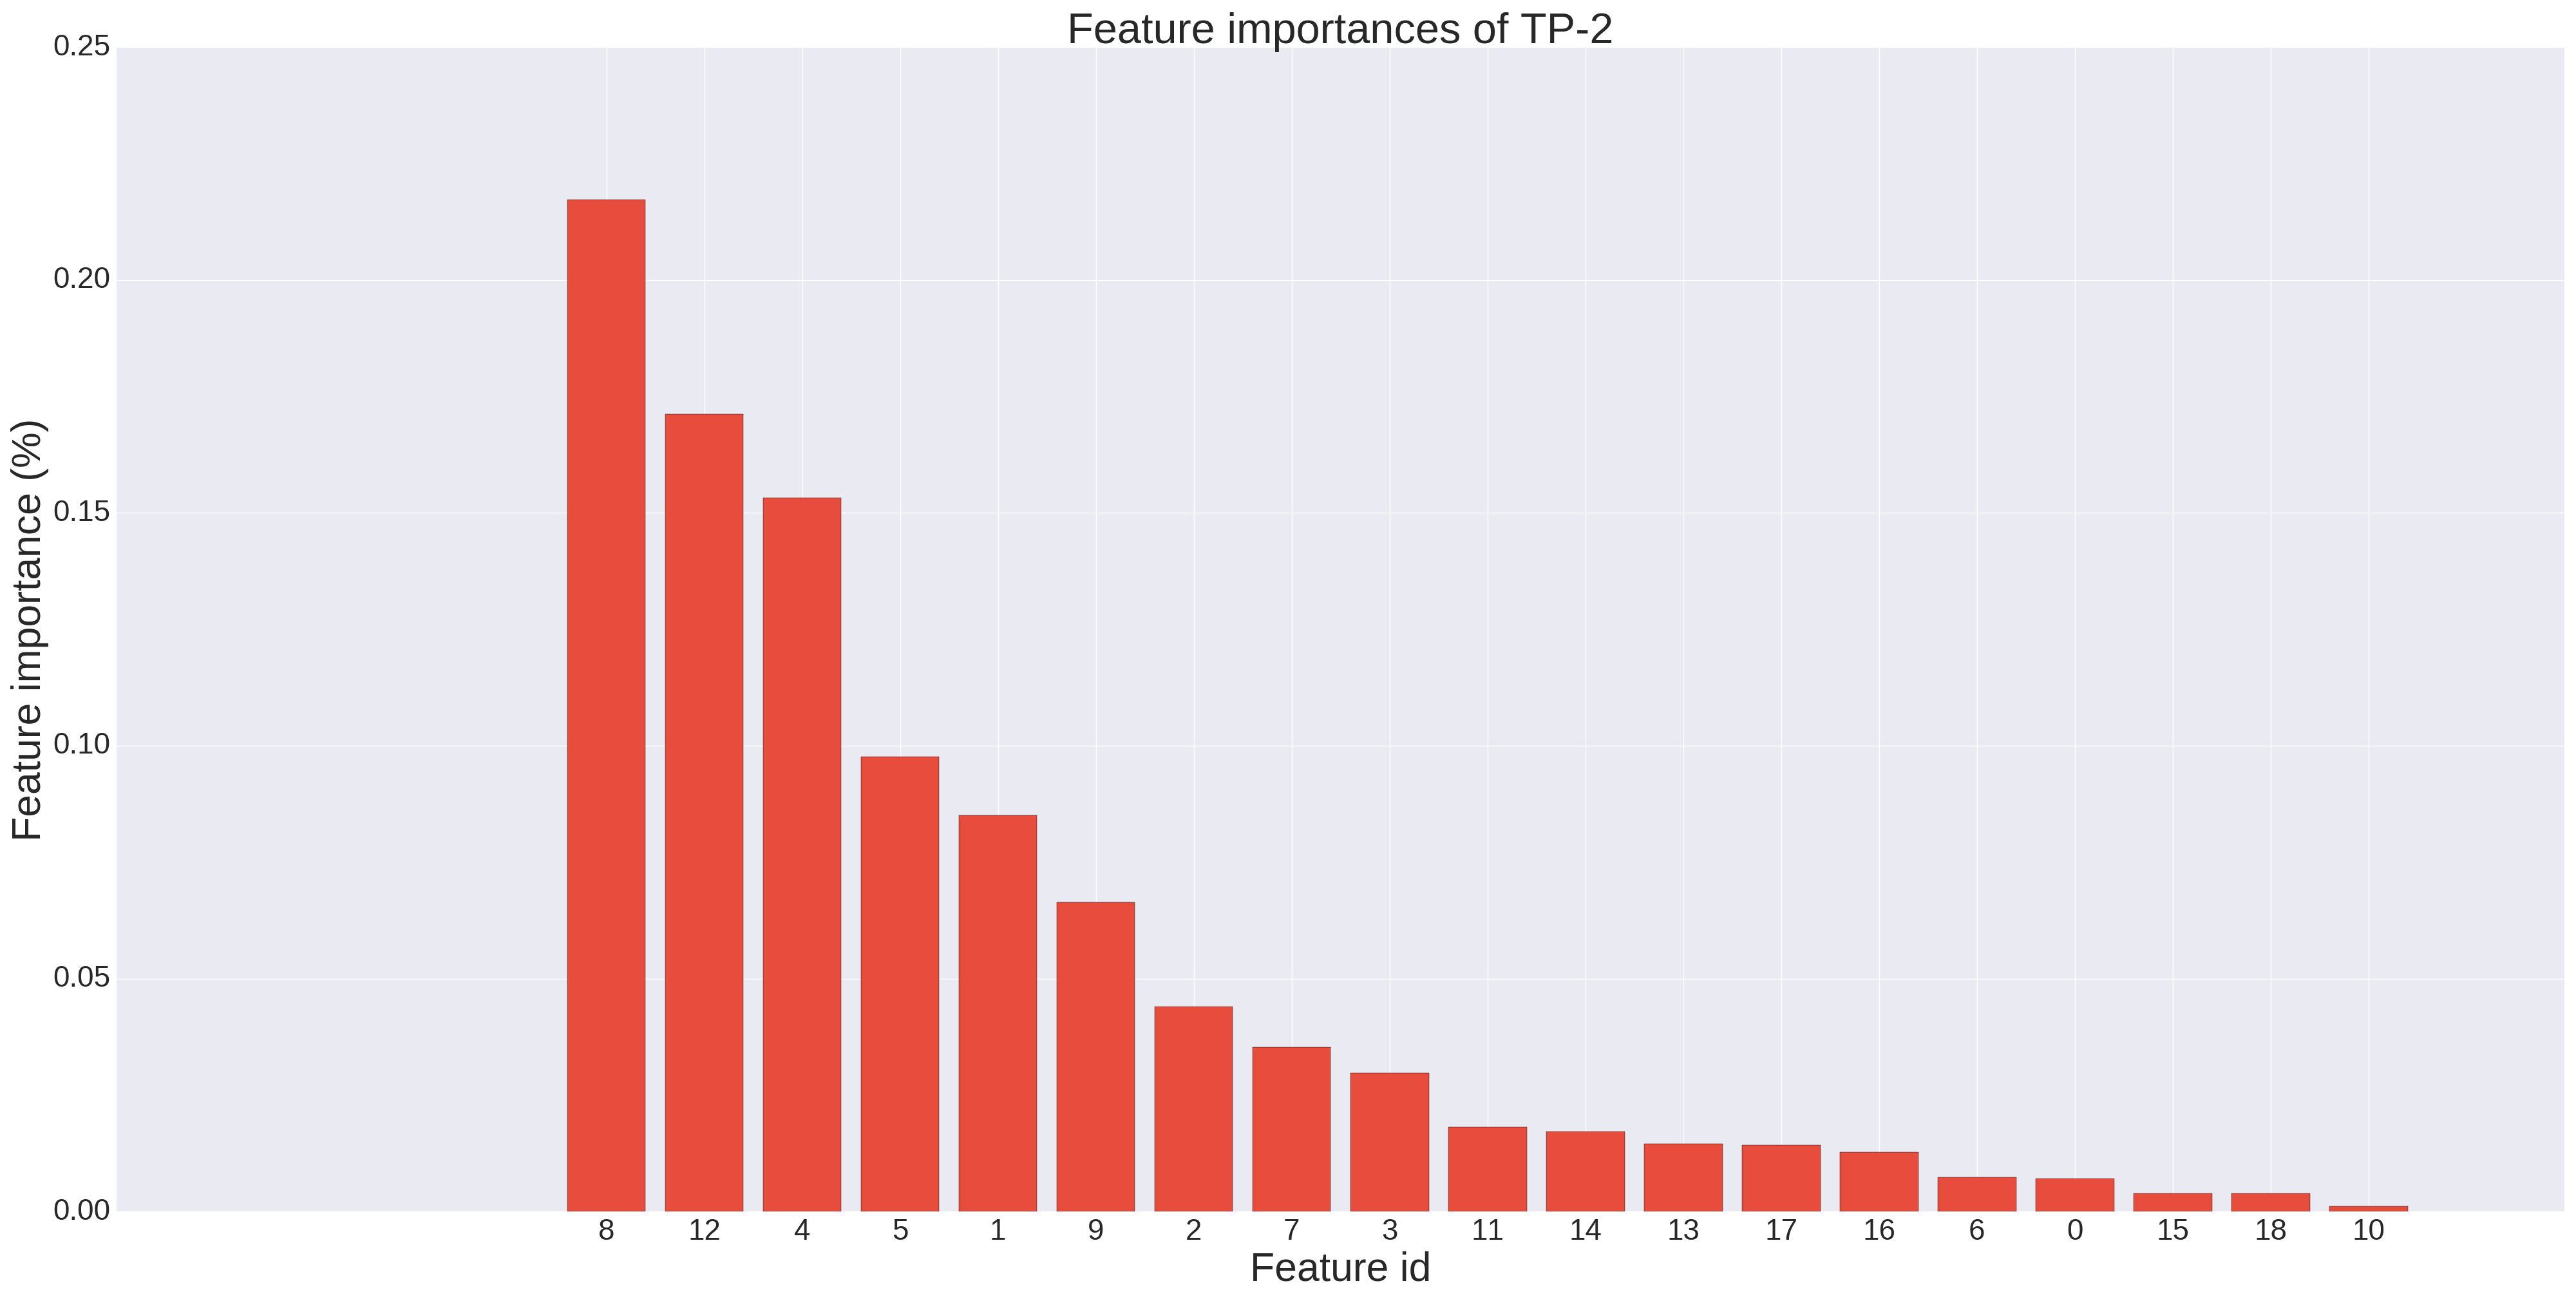
\includegraphics[scale=0.10]{feature_importance_TP2}
    \caption{Feature importances of random forest for PP2}
    \label{fig:feature_importances_tp2}
\end{figure}
For TP-2 we find features 8 (mutual co-occurrences), 12 (specificity), 4 (weighted frequency) and 5 (co-occurrences weighted) are the most important. Feature 10 (number of evenings) again contributes very little. 

Since we have not implemented the same amount of features for PP-2 and TP-2, is it difficult to compare them. Though we can see that the top 4 features are the same for PP-2 and TP-2. 

In the next plots we try to look at the differences in features between the meet and non-meets of the TP-2 dataset. We chose TP-2 because it is the filtered dataset with all of our features present.

Looking at Figure \ref{fig:feature_boxplots1} to \ref{fig:feature_boxplots5} we can see features which have very little variance like number of weekends, evenings and common travels. Co-occurrences weighted and timely arrival and leaving seems to have similar values, we can note a slightly higher mean for the class did not meet. The homophily features seems very similar as well. Diversity, weighted frequency have very extreme outliers, a large diversity signifies a user pair with a very large number of locations between them. Specificity has extreme outliers as some of the previous features. App usage similarity strangely enough seems to be more similar for the class did not meet. This could be because it does not account for popular apps used by both groups. Number of co-occurrences, mutual co-occurrences and specificity seems to have higher values for the class did meet, and two of the three also contributed most to the importances for our features.

\begin{figure}[H]
    \hspace*{-1.0cm}
    \centering
    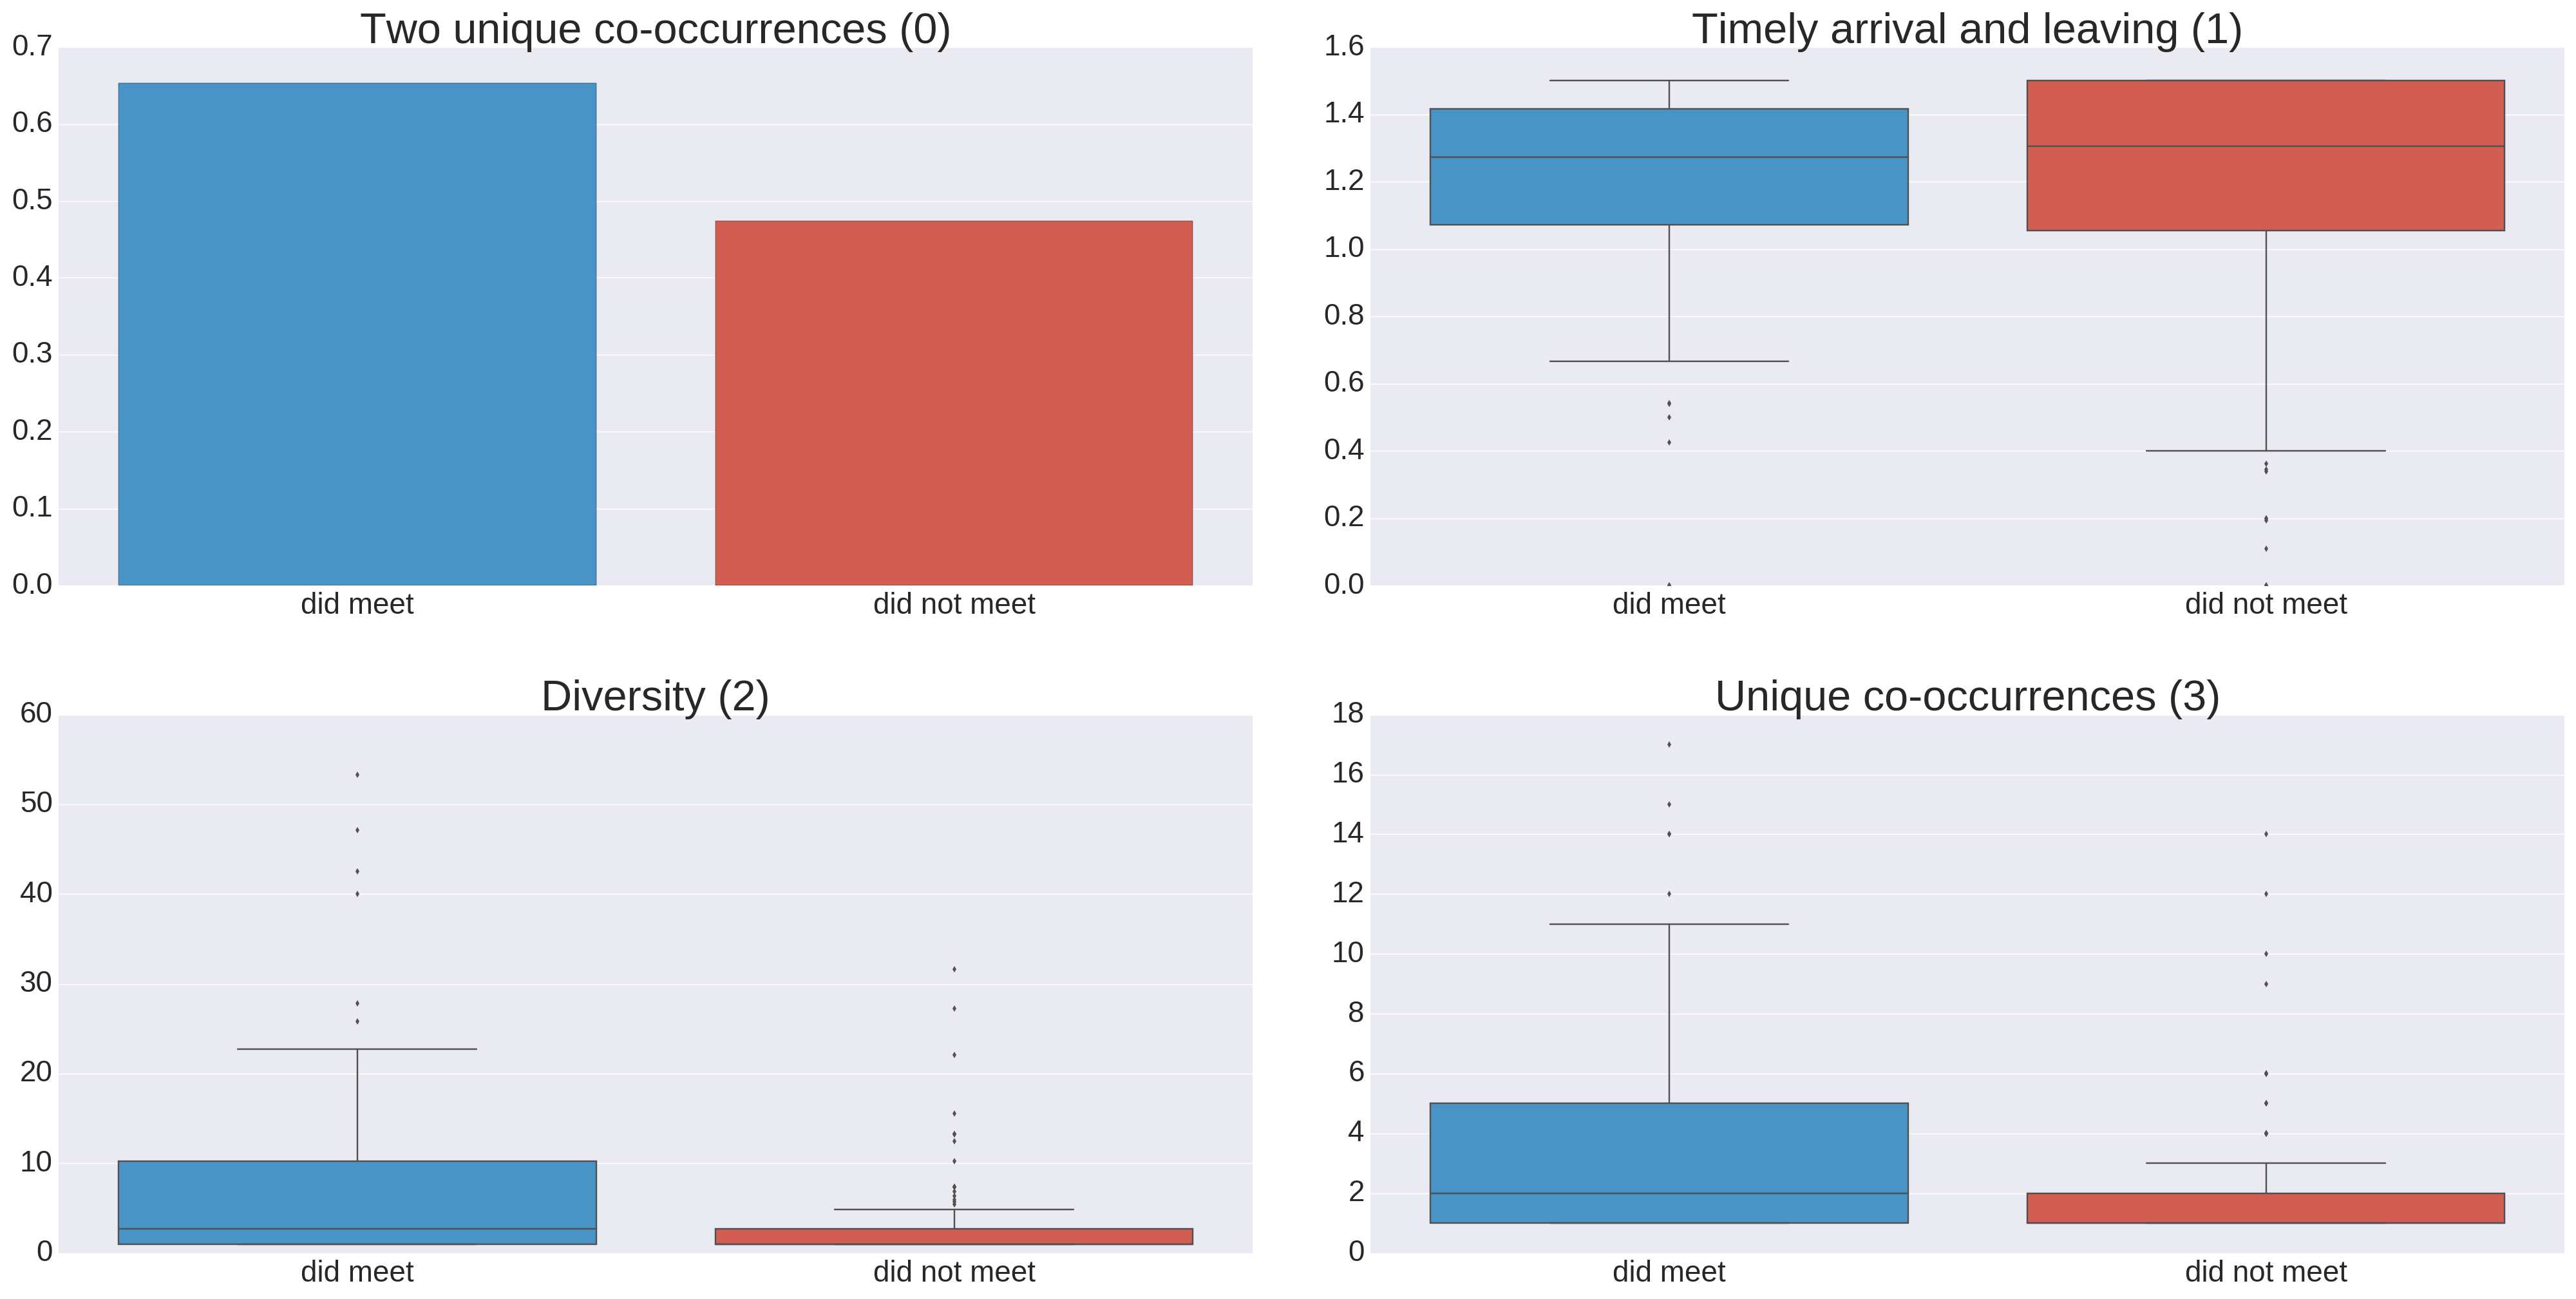
\includegraphics[scale=0.15]{feature_boxplots1_TP2}
    \caption{Boxplots of and barplots of features of TP2}
    \label{fig:feature_boxplots1}
\end{figure}

\begin{figure}[H]
    \hspace*{-1.0cm}
    \centering
    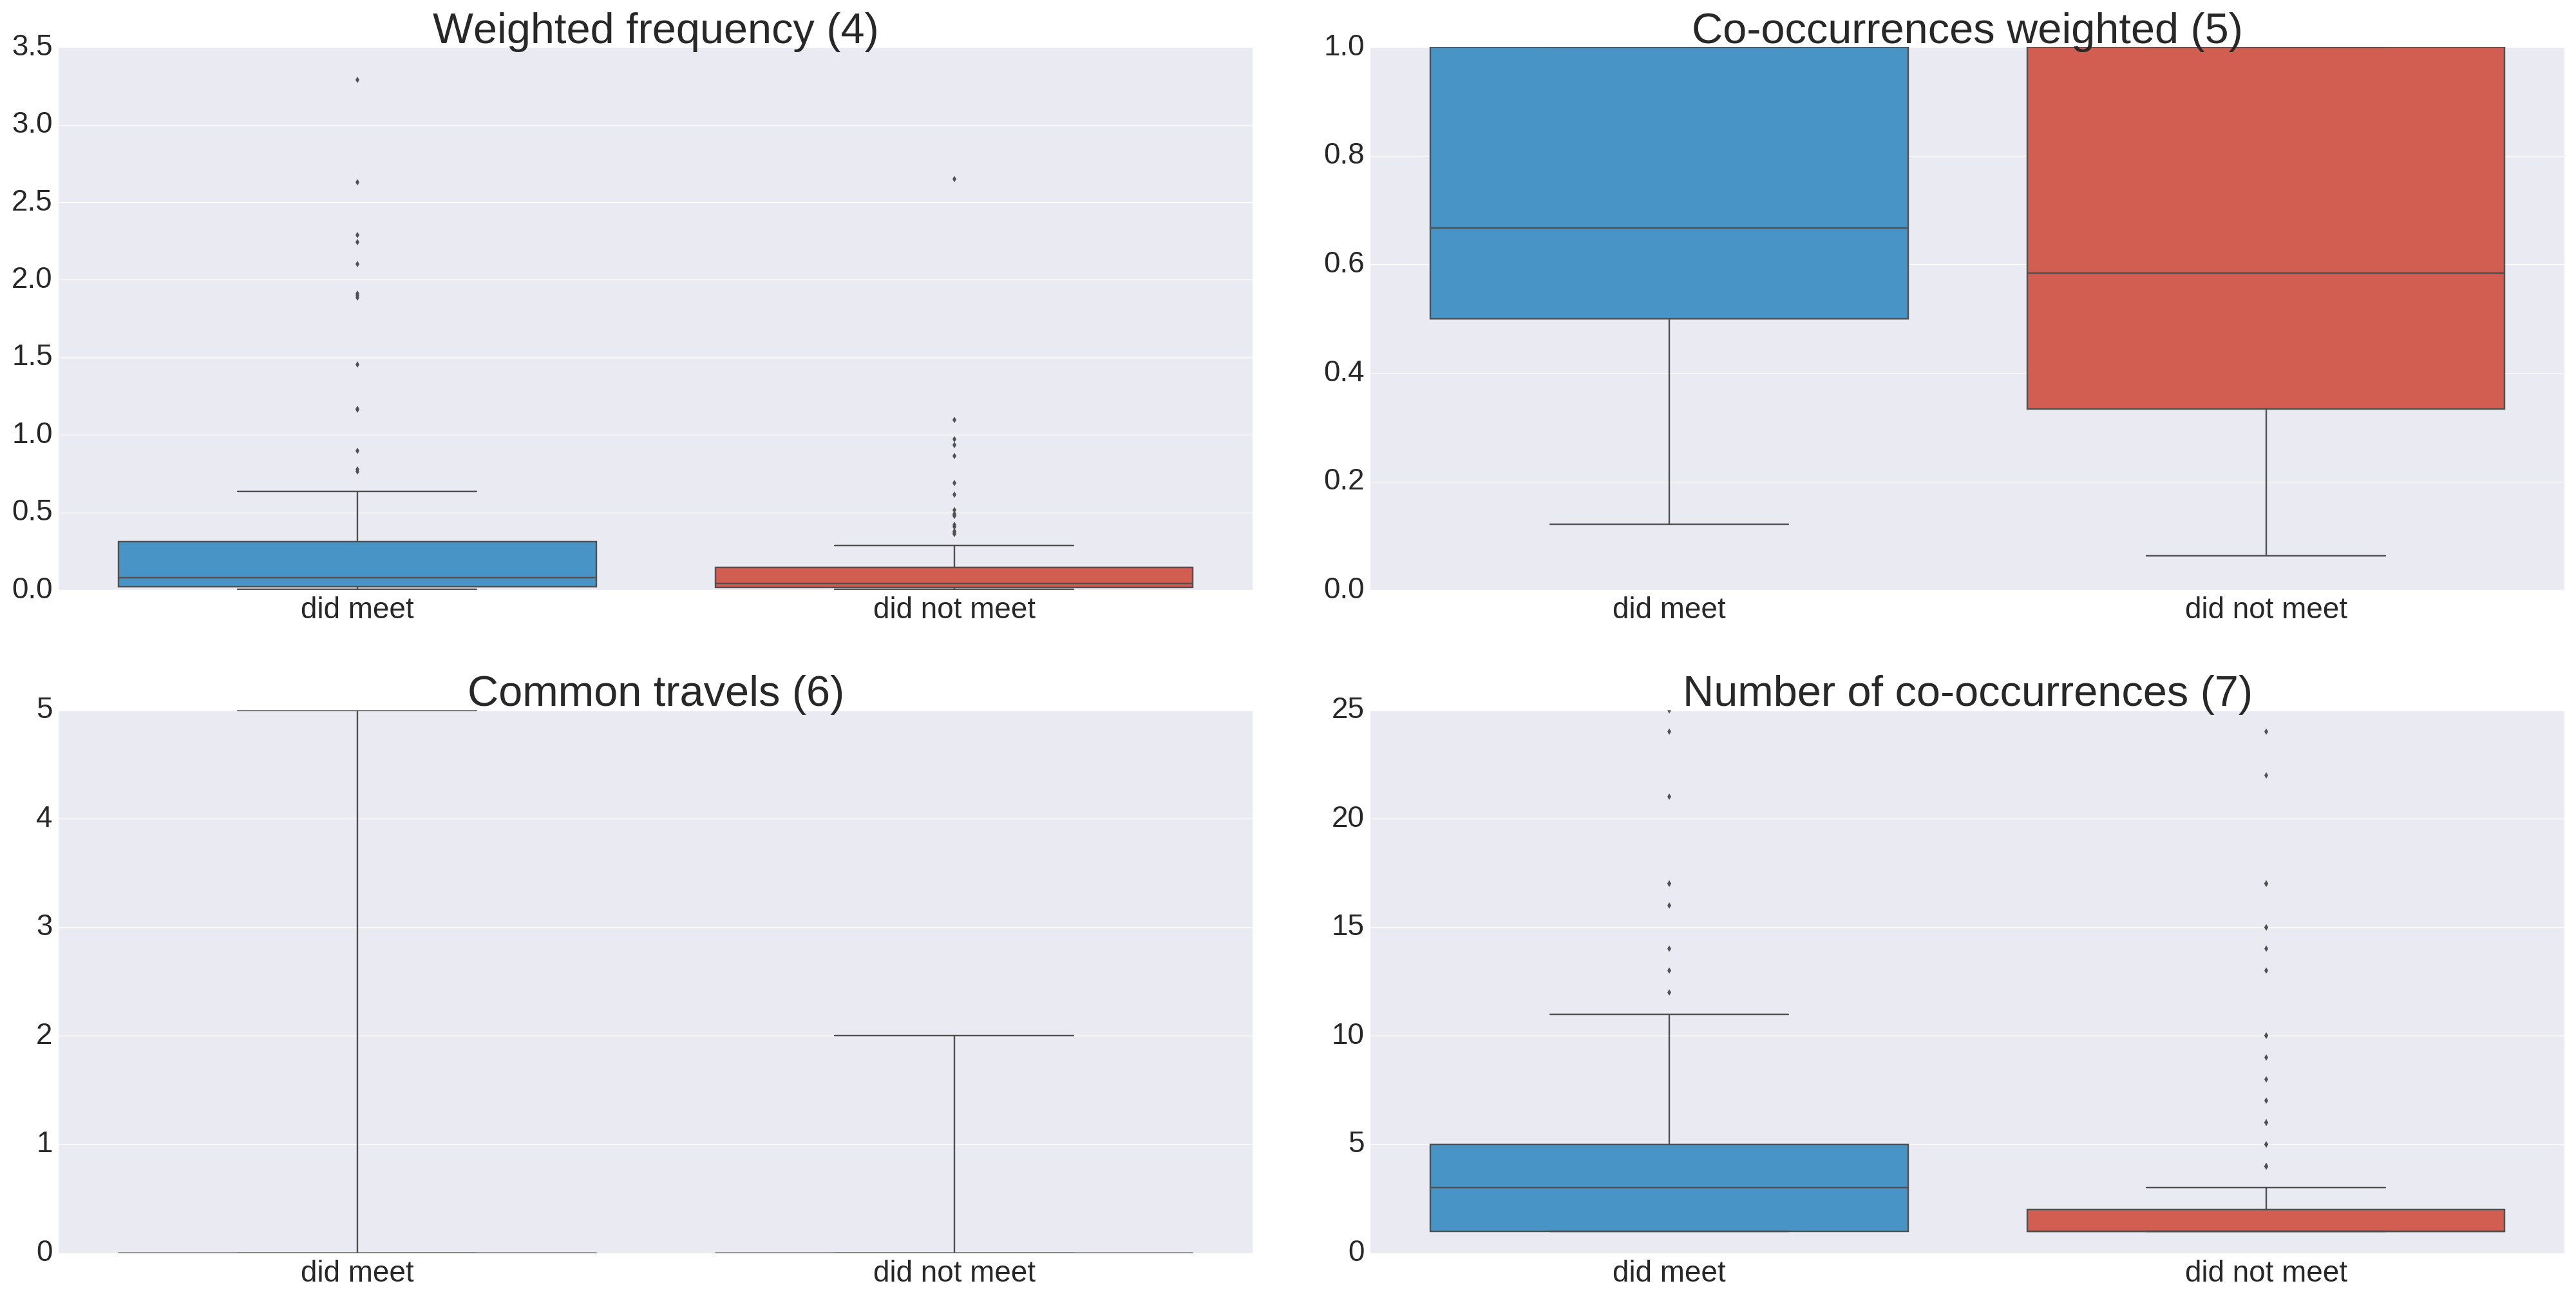
\includegraphics[scale=0.15]{feature_boxplots2_TP2}
    \caption{Boxplots of features of TP2}
    \label{fig:feature_boxplots2}
\end{figure}
\begin{figure}[H]
    \hspace*{-1.0cm}
    \centering
    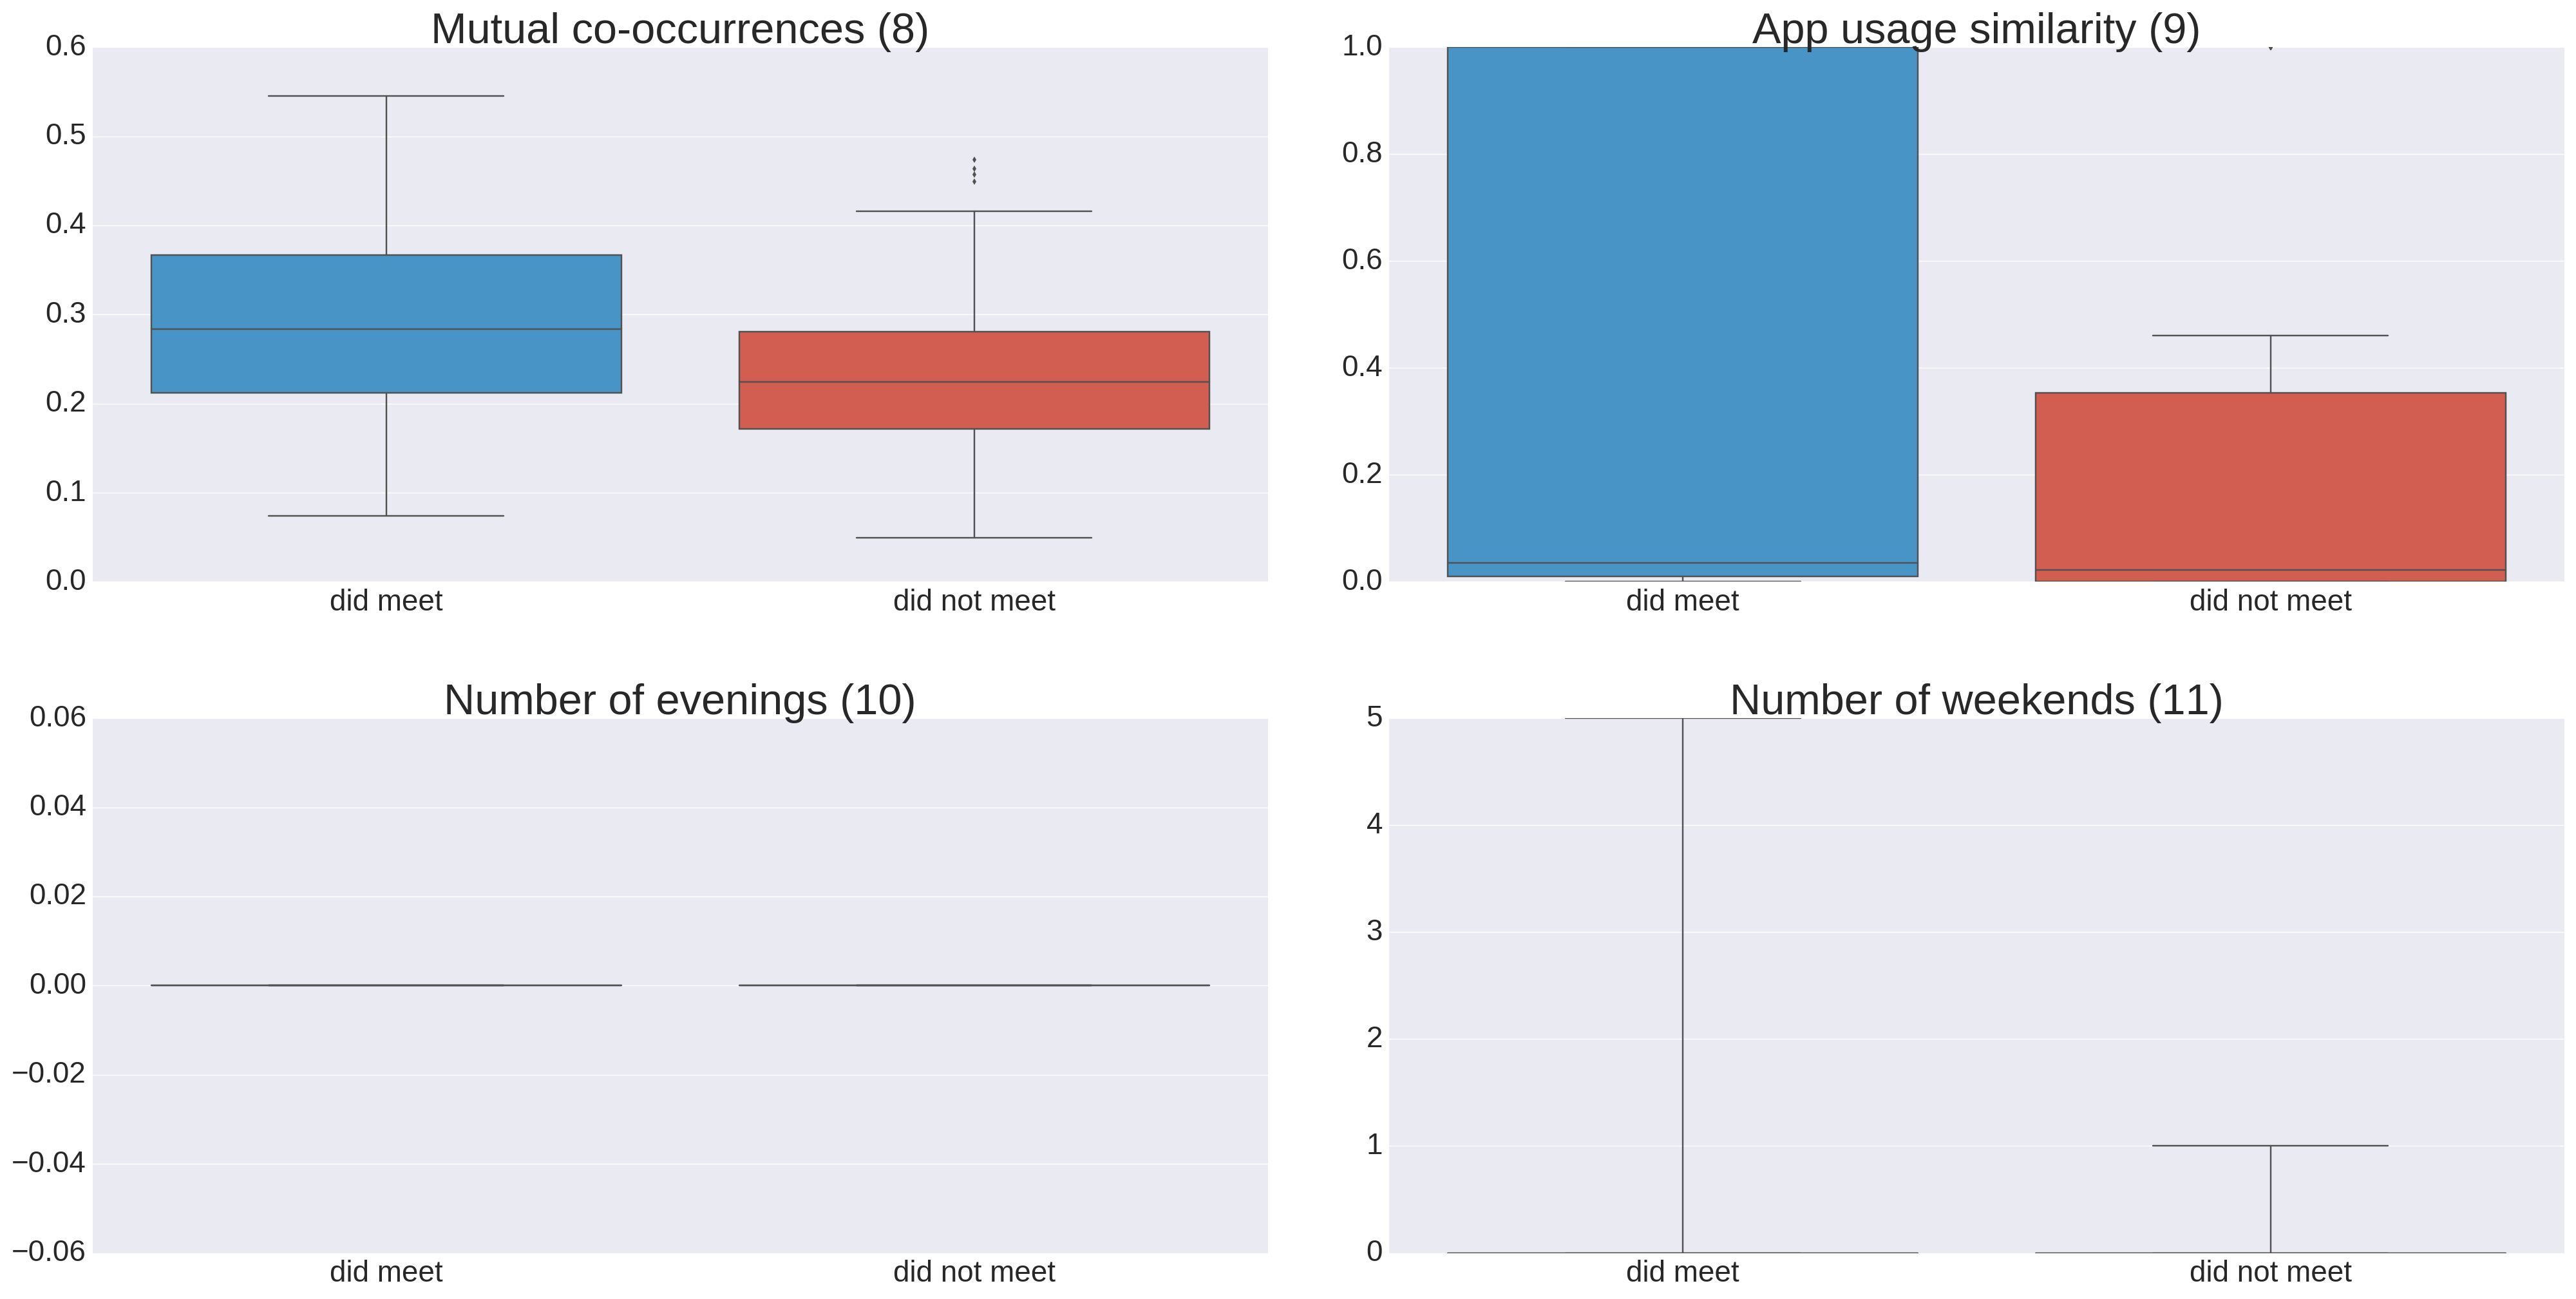
\includegraphics[scale=0.15]{feature_boxplots3_TP2}
    \caption{Boxplots and barplots of features of TP2}
    \label{fig:feature_boxplots3}
\end{figure}
\begin{figure}[H]
    \hspace*{-1.0cm}
    \centering
    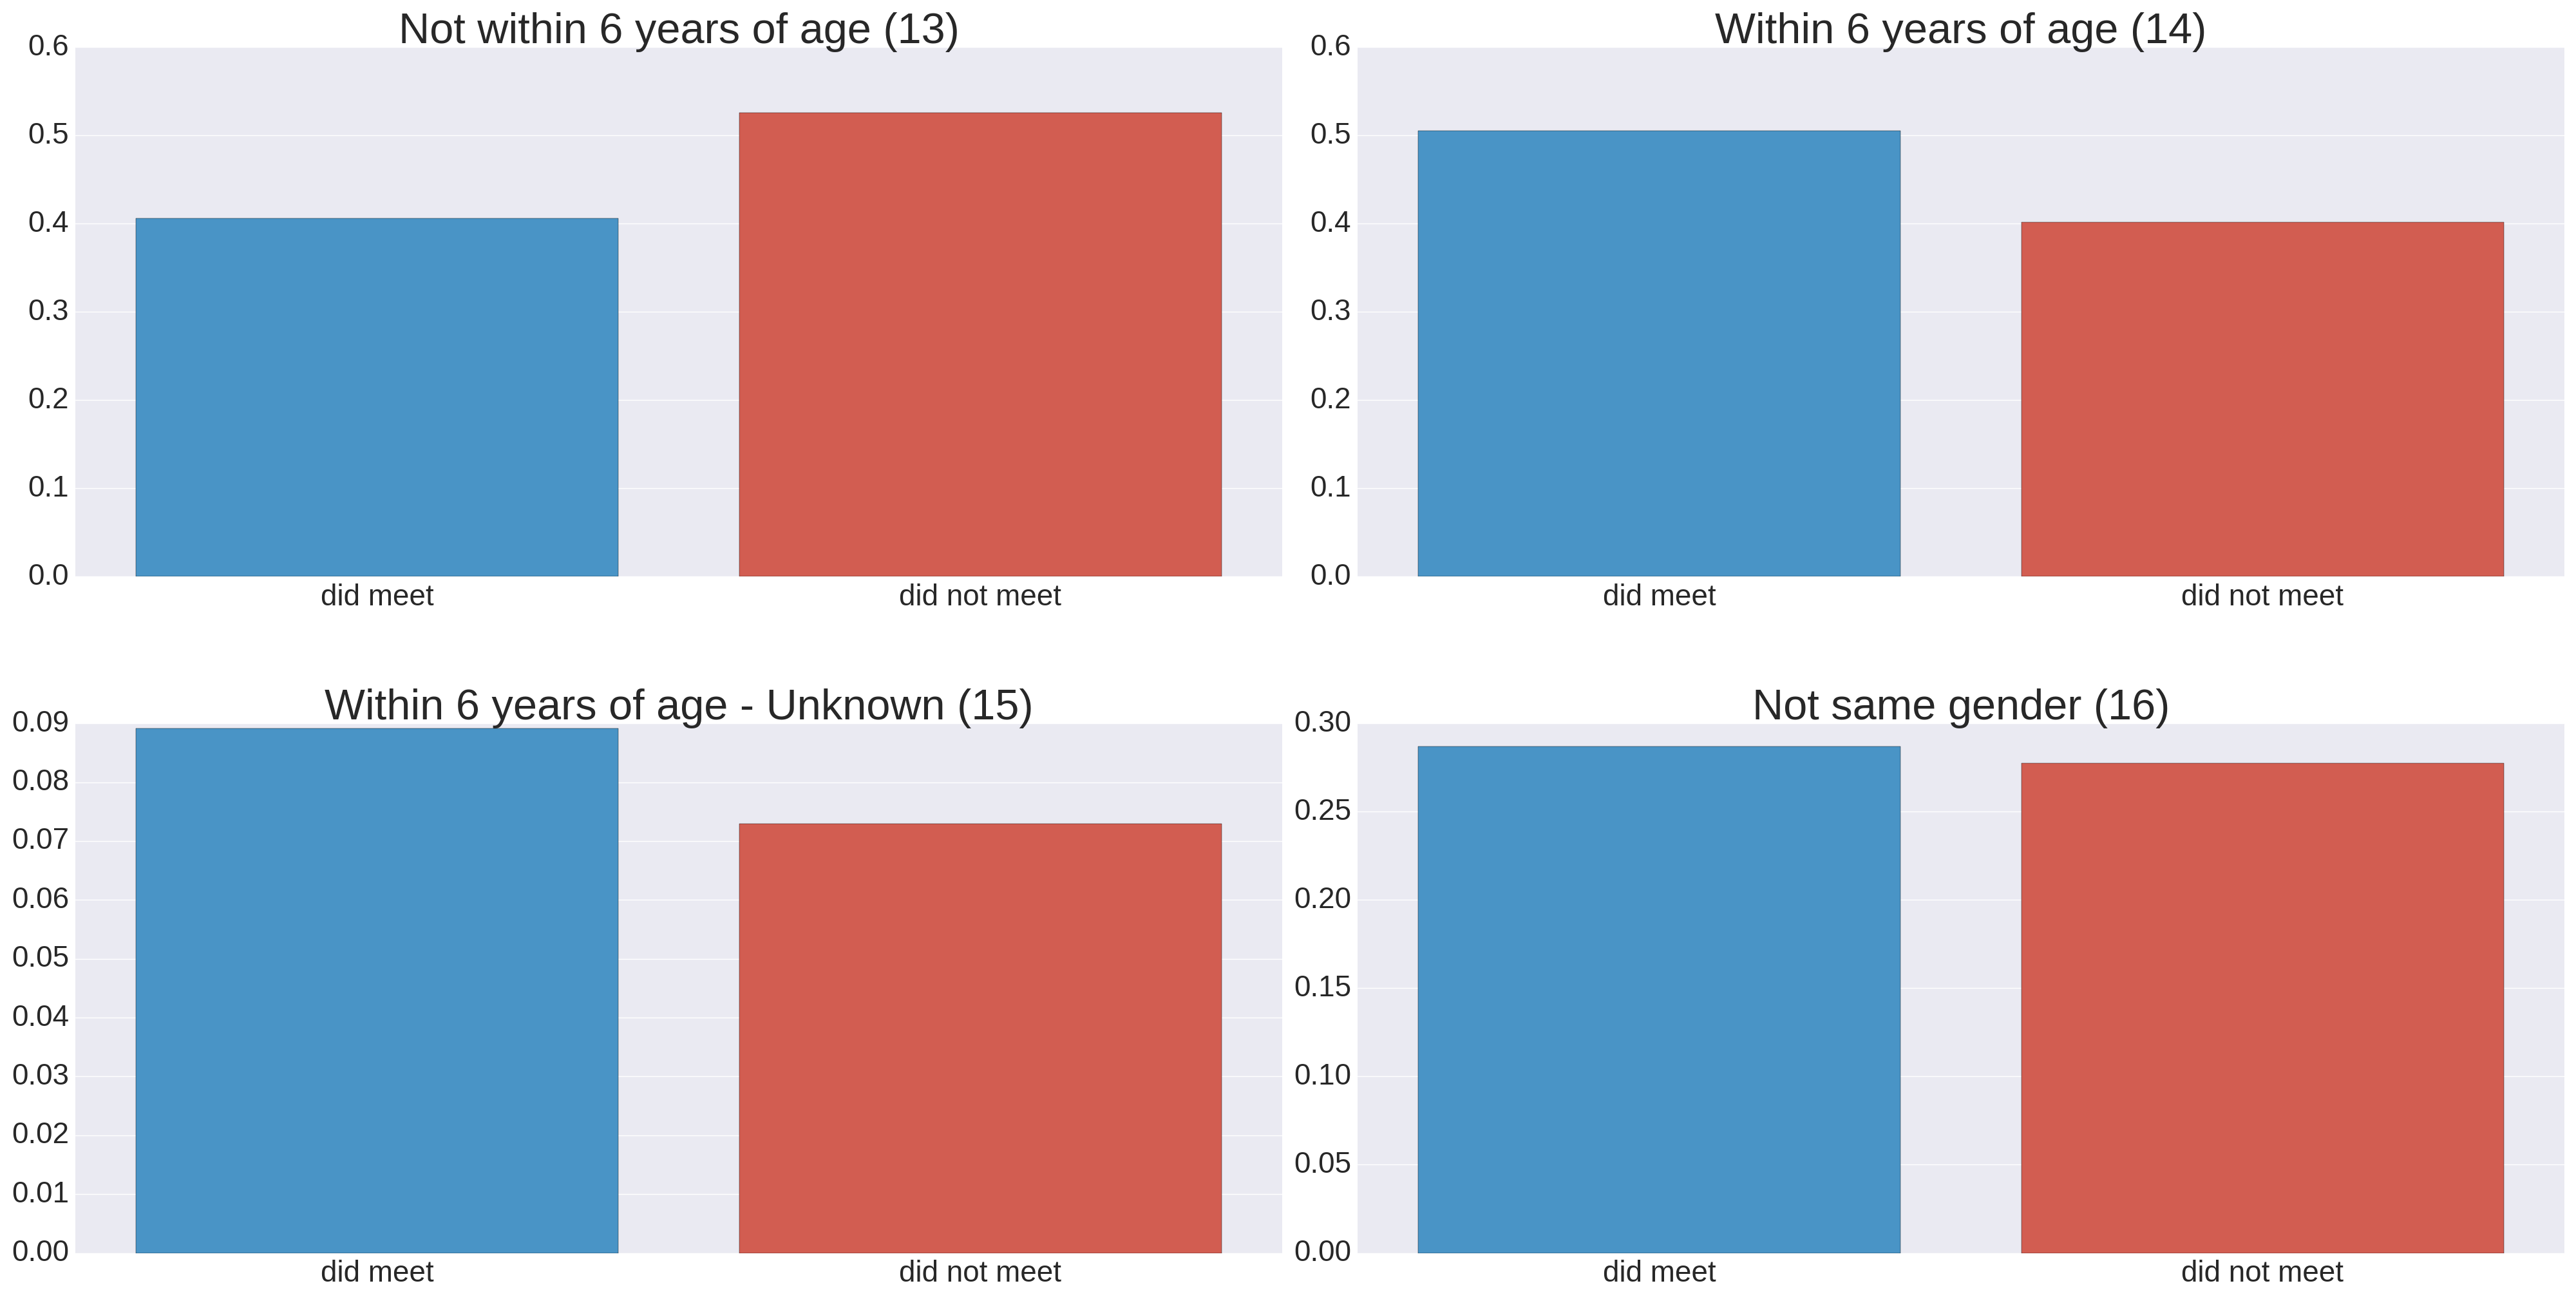
\includegraphics[scale=0.15]{feature_boxplots4_TP2}
    \caption{Boxplots of features of TP2}
    \label{fig:feature_boxplots4}
\end{figure}
\begin{figure}[H]
    \hspace*{-1.0cm}
    \centering
    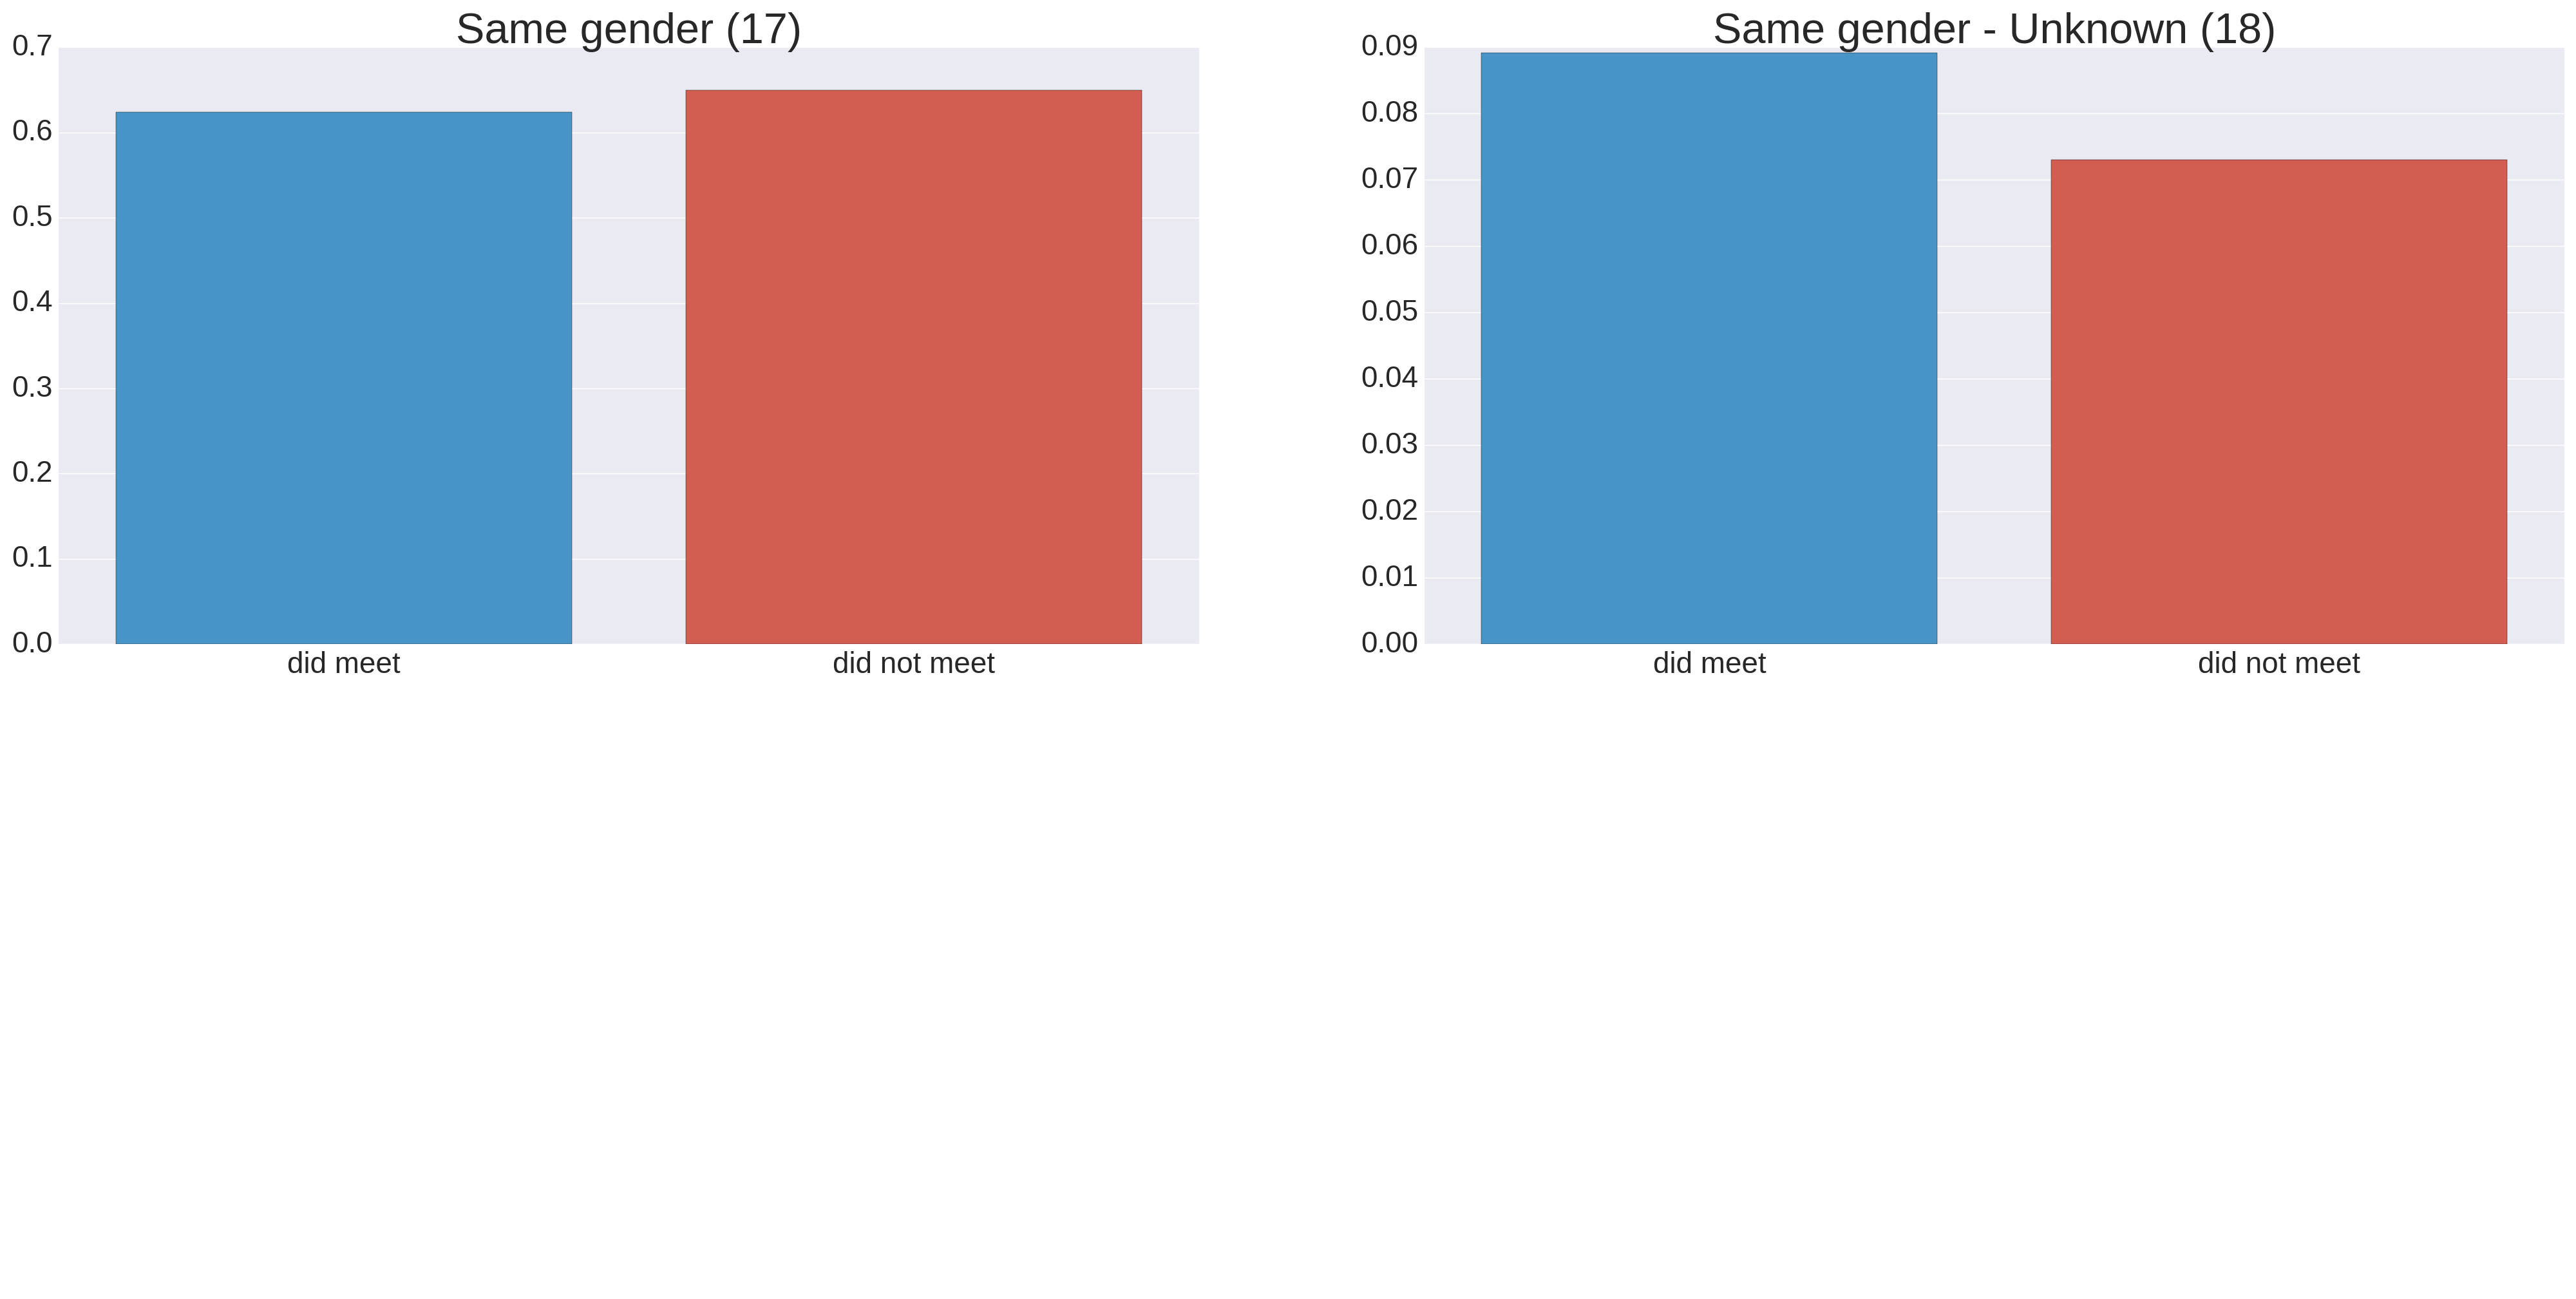
\includegraphics[scale=0.15]{feature_boxplots5_TP2}
    \caption{Boxplots of features of TP2}
    \label{fig:feature_boxplots5}
\end{figure}

\section{Summary}
In this section we will present the most important findings of our results.

The ROC AUC of the random forest compared to the baseline was higher for every dataset. This suggests however that it is simply better at predicting the negative class, did not meet, as the precision and recall scores are similar for the positive class, did meet. 
The performance of the models improve, when filtering the users on cross-occupancy, but undersampling provided no significant difference.

We found the production data made the models achieve a higher performance in terms of precision and recall compared to the test data.

We found that the most important features between datasets for the random forest models were mutual co-occurrences, specificity, co-occurrences weighted and weighted frequency.